\acao{Ação 3.2.2.2 – Trabalho técnico-social}

\phantomsection
\addcontentsline{toc}{subsection}{1. Contextualização}
\subsection*{1. Contextualização}

O trabalho técnico-social caracteriza as famílias e as condições de saneamento de cada comunidade, define o público a ser atendido e valida socialmente as soluções técnicas. Compreende também a mobilização da população, a educação sanitária e ambiental, a capacitação das lideranças locais e o estímulo à gestão participativa dos serviços, de modo que cada comunidade disponha de grupo organizado para a gestão dos sistemas (IAT, 2026a; IAT, 2026b).

A ausência de participação das famílias está associada à subutilização e ao abandono de sistemas de saneamento rural. O Programa Nacional de Saneamento Rural estabelece a educação e a participação social como um dos três eixos indissociáveis do saneamento rural, ao lado da gestão dos serviços e da tecnologia (BRASIL, 2019). Há, ainda, o risco de exclusão de famílias vulneráveis, de áreas remotas ou de comunidades tradicionais quando o levantamento se apoia apenas em cadastros preexistentes.

A ação produz as informações das quais dependem as demais. O diagnóstico subsidia a definição da captação e o projeto dos sistemas de abastecimento, identifica a situação do esgotamento sanitário em cada domicílio e reúne as adesões que dão origem às associações de saneamento rural.

\textbf{Inclui:} a mobilização dos municípios, das comunidades, das associações e dos proprietários; a busca ativa e o cadastro domiciliar; o diagnóstico coletivo e domiciliar das formas de abastecimento e de esgotamento sanitário; os critérios de enquadramento e os termos de adesão das famílias; a educação sanitária e ambiental; a capacitação das lideranças; o acompanhamento social das obras; e o relatório final.

\textbf{Não inclui:} os projetos e as obras dos sistemas nem a capacitação técnica dos operadores na pré-operação, a cargo do executor das obras de abastecimento. As duas ações atuam de forma complementar: o executor capacita os operadores, e o trabalho técnico-social trata do uso adequado e da manutenção junto às famílias.

\pendencia{Definir o item de custo da capacitação em operação e manutenção. A planilha a inclui no trabalho técnico-social; a nota técnica e o MOP de março a preveem na implantação dos sistemas.}

\textbf{Valor previsto:} R\$~6,47 milhões (empréstimo BIRD: R\$~6,47 milhões; contrapartida: R\$~0,00 milhões), conforme a planilha PSH\_CUSTO\_Consolidada.

\phantomsection
\addcontentsline{toc}{subsection}{2. Área de atuação}
\subsection*{2. Área de atuação}

A ação abrange as 83 comunidades da seleção preliminar dos sistemas de abastecimento de água, com 5.810 domicílios e cerca de 16,3 mil pessoas, que constituem também a base do esgotamento sanitário nas comunidades (Figura~\ref{mapa}). O diagnóstico confirma ou corrige a seleção preliminar: comunidades sem adesão suficiente ou sem viabilidade técnica podem ser substituídas por outras que atendam aos mesmos critérios. Em cada comunidade, as famílias atendidas são definidas por critérios sociais, territoriais e técnicos, aplicados na Etapa 5.

\phantomsection
\addcontentsline{toc}{subsection}{3. Arranjo institucional e partes interessadas}
\subsection*{3. Arranjo institucional e partes interessadas}

O IAT, por meio da DISAR, contrata a empresa, fiscaliza o contrato e valida os produtos, com a participação da SEAB, que atua junto às comunidades rurais e apoia a mobilização. A empresa contratada executa o trabalho de campo, e as prefeituras apoiam a articulação local, a divulgação e a cessão de espaços para as reuniões. A UGP acompanha a execução.

\begin{itemize}
  \item \textbf{Coexecutora:} SEAB, na mobilização e na validação dos produtos;
  \item \textbf{Intervenientes:} prefeituras; associações de moradores e lideranças locais; empresa contratada;
  \item \textbf{Público envolvido:} famílias e proprietários das comunidades selecionadas.
\end{itemize}

Os beneficiários diretos são as famílias das 83 comunidades, cerca de 16,3 mil pessoas, e as lideranças capacitadas. Os beneficiários indiretos são os municípios, que passam a dispor de cadastro atualizado do saneamento rural, aplicável a outras políticas públicas.

\phantomsection
\addcontentsline{toc}{subsection}{4. Processo de execução operacional}
\subsection*{4. Processo de execução operacional}

A ação compreende sete etapas, da contratação da empresa ao relatório final (Figura~\ref{raias-3222}). A empresa contratada executa o trabalho de campo, e as famílias formalizam a adesão na Etapa 5. Os produtos das etapas subsidiam os modelos de gestão, os projetos dos sistemas de abastecimento e o esgotamento sanitário nas comunidades.

\begin{figure}[H]
  \centering
  \caption{Fluxograma do trabalho técnico-social: entradas, etapas por responsável e saídas}\label{raias-3222}
  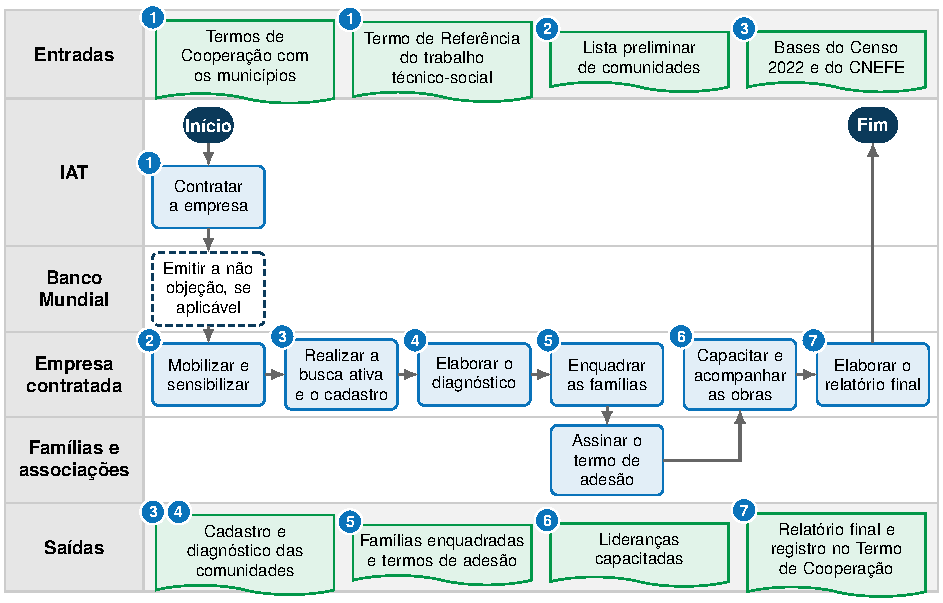
\includegraphics[width=15.96cm]{figuras/g-raias-3222.pdf}
  \fonteMOP{Fonte: IAT (2026).}
  % Texto alternativo: Fluxograma em raias do trabalho técnico-social, com uma raia por instituição, as etapas numeradas na raia do executor, as entradas no topo e as saídas na base.
\end{figure}

\phantomsection
\subsubsection*{4.1 Etapa 1: Contratação da empresa}

\textbf{Atividades:} elaboração do Termo de Referência, com escopo, produtos, prazos e perfil da equipe; publicação do edital; seleção da empresa; assinatura do contrato e emissão da ordem de serviço.

\textbf{Entradas:} Termos de Cooperação assinados com os municípios; lista preliminar de comunidades.

\textbf{Responsáveis:} IAT (executa e aprova); UGP e Banco Mundial (consultados, quando houver revisão prévia).

\textbf{Produto:} contrato assinado e ordem de serviço.

\phantomsection
\subsubsection*{4.2 Etapa 2: Mobilização e sensibilização}

\textbf{Atividades:} reuniões com as prefeituras, as associações e as lideranças; reuniões comunitárias, com linguagem acessível, para apresentação do Programa, estímulo à participação e reconhecimento do território; divulgação do Mecanismo de Queixas e Reclamações.

\textbf{Entradas:} contrato; agenda pactuada com as prefeituras.

\textbf{Responsáveis:} empresa contratada (executa); SEAB e prefeituras (consultadas); IAT (aprova).

\textbf{Produto:} plano de mobilização executado, com atas e listas de presença.

\phantomsection
\subsubsection*{4.3 Etapa 3: Busca ativa e cadastro domiciliar}

\textbf{Atividades:} visita a todos os domicílios da comunidade, inclusive em áreas remotas, sem dependência exclusiva de cadastros prévios; inventário social; cadastro domiciliar georreferenciado. O tratamento dos dados pessoais observa a Lei Geral de Proteção de Dados Pessoais (LGPD) e restringe-se às finalidades da ação (BRASIL, 2018).

\textbf{Entradas:} lista de comunidades; bases do Censo 2022 e do Cadastro Nacional de Endereços para Fins Estatísticos (CNEFE).

\textbf{Responsáveis:} empresa contratada (executa); IAT (aprova); SEAB (consultada).

\textbf{Produto:} cadastro domiciliar georreferenciado.

\phantomsection
\subsubsection*{4.4 Etapa 4: Diagnóstico coletivo e domiciliar}

\textbf{Atividades:} diagnóstico das formas atuais de abastecimento e de esgotamento sanitário, da demanda de água, da infraestrutura necessária e da viabilidade dos sistemas; levantamento das condições de cada domicílio para a solução de esgotamento sanitário; validação social das tecnologias propostas.

\textbf{Entradas:} cadastro domiciliar.

\textbf{Responsáveis:} empresa contratada (executa); IAT (aprova); SEAB (consultada).

\textbf{Produto:} diagnóstico por comunidade e por domicílio.

\phantomsection
\subsubsection*{4.5 Etapa 5: Enquadramento e adesão das famílias}

\textbf{Atividades:} aplicação dos critérios sociais, territoriais e técnicos de definição das famílias atendidas; assinatura do termo de adesão, com o compromisso de uso e manutenção adequados.

\textbf{Entradas:} diagnóstico; critérios de enquadramento aprovados pelo IAT.

\textbf{Responsáveis:} empresa contratada e famílias (executam); IAT (aprova).

\textbf{Produto:} lista de famílias enquadradas e termos de adesão assinados.

\phantomsection
\subsubsection*{4.6 Etapa 6: Educação sanitária e ambiental e acompanhamento}

\textbf{Atividades:} oficinas de educação sanitária e ambiental; capacitação das lideranças locais; apoio à organização comunitária e à constituição da associação; acompanhamento social das obras e da entrega dos sistemas.

\textbf{Entradas:} termos de adesão; cronograma das obras de abastecimento.

\textbf{Responsáveis:} empresa contratada (executa); IAT (aprova); prefeituras e SEAB (consultadas).

\textbf{Produto:} lideranças capacitadas, com listas de presença e certificados, e relatórios de acompanhamento.

\phantomsection
\subsubsection*{4.7 Etapa 7: Relatório final}

\textbf{Atividades:} consolidação dos resultados; elaboração do relatório final; registro da conclusão da etapa no Termo de Cooperação.

\textbf{Entradas:} produtos das Etapas 2 a 6.

\textbf{Responsáveis:} empresa contratada (executa); SEAB (consultada na validação); IAT (aprova).

\pendencia{A nota técnica prevê a validação conjunta do relatório final. Na matriz, a SEAB figura como C (consultada antes da aprovação), porque o Guia de Identidade Visual admite um único A por etapa; confirmar.}

\textbf{Produto:} relatório final aprovado.

\phantomsection
\subsubsection*{4.8 Modalidade de execução}

O item de custo é o trabalho técnico e social: 36 profissionais-mês a R\$~179.835,30, no total de R\$~6,47 milhões, com recursos do empréstimo do BIRD. A execução ocorre mediante licitação de serviços, conforme o Caderno AQ, e o número de lotes é definido no Plano de Aquisições.

\phantomsection
\addcontentsline{toc}{subsection}{5. Matriz de responsabilidades}
\subsection*{5. Matriz de responsabilidades}

O Quadro~\ref{raci-3222} apresenta o papel de cada parte em cada etapa.

\begin{quadro}[H]
  \caption{Matriz de responsabilidades do trabalho técnico-social}\label{raci-3222}
  \footnotesize\renewcommand{\arraystretch}{1.25}\setlength{\tabcolsep}{3pt}
  \begin{tabular}{>{\raggedright\arraybackslash}p{\dimexpr 0.2536\linewidth-2\tabcolsep\relax}>{\centering\arraybackslash}p{\dimexpr 0.0882\linewidth-2\tabcolsep\relax}>{\centering\arraybackslash}p{\dimexpr 0.0882\linewidth-2\tabcolsep\relax}>{\centering\arraybackslash}p{\dimexpr 0.0882\linewidth-2\tabcolsep\relax}>{\centering\arraybackslash}p{\dimexpr 0.0882\linewidth-2\tabcolsep\relax}>{\centering\arraybackslash}p{\dimexpr 0.0882\linewidth-2\tabcolsep\relax}>{\centering\arraybackslash}p{\dimexpr 0.0882\linewidth-2\tabcolsep\relax}>{\centering\arraybackslash}p{\dimexpr 0.0882\linewidth-2\tabcolsep\relax}>{\centering\arraybackslash}p{\dimexpr 0.1291\linewidth-2\tabcolsep\relax}}
    \rowcolor{azulEscuro}\textcolor{white}{\textbf{Parte}} & \textcolor{white}{\textbf{E1}} & \textcolor{white}{\textbf{E2}} & \textcolor{white}{\textbf{E3}} & \textcolor{white}{\textbf{E4}} & \textcolor{white}{\textbf{E5}} & \textcolor{white}{\textbf{E6}} & \textcolor{white}{\textbf{E7}} & \textcolor{white}{\textbf{Produto final}} \\
    IAT & \raci{R} \raci{A} & \raci{A} & \raci{A} & \raci{A} & \raci{A} & \raci{A} & \raci{A} & \raci{A} \\ \arrayrulecolor{cinza20}\hline
    \rowcolor{cinza5}SEAB & – & \raci{C} & \raci{C} & \raci{C} & \raci{C} & \raci{C} & \raci{C} & \raci{C} \\ \arrayrulecolor{cinza20}\hline
    Empresa contratada & – & \raci{R} & \raci{R} & \raci{R} & \raci{R} & \raci{R} & \raci{R} & \raci{R} \\ \arrayrulecolor{cinza20}\hline
    \rowcolor{cinza5}Prefeituras & \raci{I} & \raci{C} & \raci{I} & \raci{I} & \raci{I} & \raci{C} & \raci{I} & \raci{I} \\ \arrayrulecolor{cinza20}\hline
    Famílias e associações & – & \raci{C} & \raci{C} & \raci{C} & \raci{R} & \raci{C} & \raci{I} & \raci{I} \\ \arrayrulecolor{cinza20}\hline
    \rowcolor{cinza5}UGP & \raci{C} & \raci{I} & \raci{I} & \raci{I} & \raci{I} & \raci{I} & \raci{I} & \raci{I} \\ \arrayrulecolor{cinza20}\hline
    Banco Mundial & \raci{C} & – & – & – & – & – & – & – \\ \noalign{\global\arrayrulewidth=1pt}\arrayrulecolor{azulEscuro}\hline\noalign{\global\arrayrulewidth=0.4pt}
  \end{tabular}
  \fonteMOP{Fonte: IAT (2026).}
  \notaMOP{Nota: E1 a E7 correspondem às Etapas 1 a 7 do item 4. \raci{R} executa (pode haver mais de um); \raci{A} aprova ou valida o produto (um por etapa); \raci{C} é consultado previamente; \raci{I} é informado posteriormente. Produto final: cadastro, diagnóstico e termos de adesão das 83 comunidades.}
\end{quadro}

\phantomsection
\addcontentsline{toc}{subsection}{6. Metas, indicadores e comprovação}
\subsection*{6. Metas, indicadores e comprovação}

A meta física é expressa em profissionais-mês e concentra-se entre 2027 e 2030 (Quadro~\ref{metas-3222}), pois o diagnóstico deve estar concluído antes dos projetos e das obras.

\begin{quadro}[H]
  \caption{Metas anuais do trabalho técnico-social}\label{metas-3222}
  \footnotesize\renewcommand{\arraystretch}{1.25}\setlength{\tabcolsep}{3pt}
  \begin{tabular}{>{\raggedright\arraybackslash}p{\dimexpr 0.2095\linewidth-2\tabcolsep\relax}>{\raggedright\arraybackslash}p{\dimexpr 0.1268\linewidth-2\tabcolsep\relax}>{\raggedleft\arraybackslash}p{\dimexpr 0.0794\linewidth-2\tabcolsep\relax}>{\raggedleft\arraybackslash}p{\dimexpr 0.0794\linewidth-2\tabcolsep\relax}>{\raggedleft\arraybackslash}p{\dimexpr 0.0794\linewidth-2\tabcolsep\relax}>{\raggedleft\arraybackslash}p{\dimexpr 0.0794\linewidth-2\tabcolsep\relax}>{\raggedleft\arraybackslash}p{\dimexpr 0.0794\linewidth-2\tabcolsep\relax}>{\raggedleft\arraybackslash}p{\dimexpr 0.0794\linewidth-2\tabcolsep\relax}>{\raggedleft\arraybackslash}p{\dimexpr 0.0794\linewidth-2\tabcolsep\relax}>{\raggedleft\arraybackslash}p{\dimexpr 0.1081\linewidth-2\tabcolsep\relax}}
    \rowcolor{azulEscuro}\textcolor{white}{\textbf{Produto}} & \textcolor{white}{\textbf{Unidade}} & \centering\arraybackslash \textcolor{white}{\textbf{Ano 1}} & \centering\arraybackslash \textcolor{white}{\textbf{Ano 2}} & \centering\arraybackslash \textcolor{white}{\textbf{Ano 3}} & \centering\arraybackslash \textcolor{white}{\textbf{Ano 4}} & \centering\arraybackslash \textcolor{white}{\textbf{Ano 5}} & \centering\arraybackslash \textcolor{white}{\textbf{Ano 6}} & \centering\arraybackslash \textcolor{white}{\textbf{Ano 7}} & \centering\arraybackslash \textcolor{white}{\textbf{Total}} \\
    Trabalho técnico e social & prof.-mês & 6 & 12 & 12 & 6 & – & – & – & 36 \\ \noalign{\global\arrayrulewidth=1pt}\arrayrulecolor{azulEscuro}\hline\noalign{\global\arrayrulewidth=0.4pt}
  \end{tabular}
  \fonteMOP{Fonte: Planilha PSH\_CUSTO\_Consolidada, versão v2408 (PARANÁ, 2026).}
  \notaMOP{Nota: Ano 1 = 2027 e Ano 7 = 2033. Prof.-mês = profissionais-mês.}
\end{quadro}

O Quadro~\ref{ind-3222} reúne os indicadores de andamento da ação, apurados por comunidade.

\begin{quadro}[H]
  \caption{Indicadores do trabalho técnico-social}\label{ind-3222}
  \footnotesize\renewcommand{\arraystretch}{1.25}\setlength{\tabcolsep}{3pt}
  \begin{tabular}{>{\raggedright\arraybackslash}p{\dimexpr 0.3165\linewidth-2\tabcolsep\relax}>{\raggedright\arraybackslash}p{\dimexpr 0.1378\linewidth-2\tabcolsep\relax}>{\raggedleft\arraybackslash}p{\dimexpr 0.1102\linewidth-2\tabcolsep\relax}>{\raggedleft\arraybackslash}p{\dimexpr 0.1599\linewidth-2\tabcolsep\relax}>{\raggedright\arraybackslash}p{\dimexpr 0.2756\linewidth-2\tabcolsep\relax}}
    \rowcolor{azulEscuro}\textcolor{white}{\textbf{Indicador}} & \textcolor{white}{\textbf{Unidade}} & \centering\arraybackslash \textcolor{white}{\textbf{Linha de base (2025)}} & \centering\arraybackslash \textcolor{white}{\textbf{Meta}} & \textcolor{white}{\textbf{Frequência e fonte dos dados}} \\
    Comunidades com diagnóstico aprovado & comunidades & 0 & 83 & Por lote; IAT \\ \arrayrulecolor{cinza20}\hline
    \rowcolor{cinza5}Domicílios cadastrados & domicílios & 0 & 5.810 & Por lote; cadastro domiciliar \\ \arrayrulecolor{cinza20}\hline
    Famílias com termo de adesão assinado & famílias & 0 & a definir no diagnóstico & Por lote; IAT \\ \arrayrulecolor{cinza20}\hline
    \rowcolor{cinza5}Lideranças e moradores capacitados & pessoas & 0 & a definir no plano de trabalho & Semestral; listas de presença \\ \noalign{\global\arrayrulewidth=1pt}\arrayrulecolor{azulEscuro}\hline\noalign{\global\arrayrulewidth=0.4pt}
  \end{tabular}
  \fonteMOP{Fonte: IAT (2026).}
\end{quadro}

\pendencia{Definir as metas de famílias aderidas e de pessoas capacitadas no plano de trabalho da empresa contratada.}

Os critérios de aceite e as evidências constam do Quadro~\ref{aceite-3222}. O relatório final, aprovado pelo IAT após consulta à SEAB, constitui a evidência de conclusão de cada lote e registra a conclusão da etapa no Termo de Cooperação.

\begin{quadro}[H]
  \caption{Critérios de aceite e evidências do trabalho técnico-social}\label{aceite-3222}
  \footnotesize\renewcommand{\arraystretch}{1.25}\setlength{\tabcolsep}{5pt}
  \begin{tabular}{>{\raggedright\arraybackslash}p{\dimexpr 0.2150\linewidth-2\tabcolsep\relax}>{\raggedright\arraybackslash}p{\dimexpr 0.3386\linewidth-2\tabcolsep\relax}>{\raggedright\arraybackslash}p{\dimexpr 0.2921\linewidth-2\tabcolsep\relax}>{\raggedright\arraybackslash}p{\dimexpr 0.1543\linewidth-2\tabcolsep\relax}}
    \rowcolor{azulEscuro}\textcolor{white}{\textbf{Produto}} & \textcolor{white}{\textbf{Critério de aceite}} & \textcolor{white}{\textbf{Evidência de comprovação}} & \textcolor{white}{\textbf{Responsável pela validação}} \\
    Plano de trabalho & Metodologia, cronograma e equipe compatíveis com o Termo de Referência & Plano aprovado & IAT \\ \arrayrulecolor{cinza20}\hline
    \rowcolor{cinza5}Cadastro domiciliar & Todos os domicílios da comunidade visitados e georreferenciados; dados tratados conforme a LGPD & Base do cadastro; relatório de campo & IAT \\ \arrayrulecolor{cinza20}\hline
    Diagnóstico & Condições de abastecimento e de esgotamento sanitário descritas por comunidade e por domicílio & Relatório de diagnóstico & IAT \\ \arrayrulecolor{cinza20}\hline
    \rowcolor{cinza5}Termos de adesão & Assinados pelas famílias enquadradas & Termos assinados & IAT \\ \arrayrulecolor{cinza20}\hline
    Capacitação & Conteúdo do plano de educação sanitária e ambiental cumprido & Listas de presença e certificados & IAT \\ \arrayrulecolor{cinza20}\hline
    \rowcolor{cinza5}Relatório final & Consolida os produtos e é aprovado & Relatório final; registro no Termo de Cooperação & IAT, após consulta à SEAB \\ \noalign{\global\arrayrulewidth=1pt}\arrayrulecolor{azulEscuro}\hline\noalign{\global\arrayrulewidth=0.4pt}
  \end{tabular}
  \fonteMOP{Fonte: IAT (2026).}
\end{quadro}

\phantomsection
\addcontentsline{toc}{subsection}{7. Gestão de riscos e impactos ambientais e sociais}
\subsection*{7. Gestão de riscos e impactos ambientais e sociais}

A ação não envolve obras. Os riscos concentram-se na exclusão de famílias, na consulta inadequada a comunidades tradicionais, nas condições de trabalho da equipe de campo e no tratamento dos dados pessoais do cadastro. O Quadro~\ref{nas-3222} indica as NAS aplicáveis e as medidas; as NAS 3, 4, 5, 6 e 8 não se aplicam à ação.

\begin{quadro}[H]
  \caption{Aplicação das Normas Ambientais e Sociais ao trabalho técnico-social}\label{nas-3222}
  \footnotesize\renewcommand{\arraystretch}{1.25}\setlength{\tabcolsep}{5pt}
  \begin{tabular}{>{\raggedright\arraybackslash}p{\dimexpr 0.1874\linewidth-2\tabcolsep\relax}>{\raggedright\arraybackslash}p{\dimexpr 0.3716\linewidth-2\tabcolsep\relax}>{\raggedright\arraybackslash}p{\dimexpr 0.4410\linewidth-2\tabcolsep\relax}}
    \rowcolor{azulEscuro}\textcolor{white}{\textbf{NAS}} & \textcolor{white}{\textbf{Aplicação à ação}} & \textcolor{white}{\textbf{Medidas e instrumentos}} \\
    NAS 1 – Avaliação e gestão de riscos & Risco de exclusão de famílias vulneráveis ou de áreas remotas & Busca ativa em todos os domicílios; aplicação rigorosa dos critérios de vulnerabilidade social (MGAS) \\ \arrayrulecolor{cinza20}\hline
    \rowcolor{cinza5}NAS 2 – Condições de trabalho & Equipe de campo da empresa contratada & Cláusulas trabalhistas e de segurança nos deslocamentos; Procedimentos de Gestão de Mão de Obra \\ \arrayrulecolor{cinza20}\hline
    NAS 7 – Povos indígenas e comunidades tradicionais & Comunidades tradicionais nas áreas selecionadas & Consulta culturalmente adequada, com participação das lideranças (MGAS e PEPI) \\ \arrayrulecolor{cinza20}\hline
    \rowcolor{cinza5}NAS 10 – Engajamento das partes interessadas & Toda a ação, por constituir o principal canal de diálogo com as famílias & Reuniões com linguagem acessível; registro das consultas; divulgação e acompanhamento do Mecanismo de Queixas e Reclamações (PEPI e MQR) \\ \noalign{\global\arrayrulewidth=1pt}\arrayrulecolor{azulEscuro}\hline\noalign{\global\arrayrulewidth=0.4pt}
  \end{tabular}
  \fonteMOP{Fonte: IAT (2026), com base nos instrumentos do Caderno AS.}
  \notaMOP{Nota: o cadastro domiciliar observa a Lei Geral de Proteção de Dados Pessoais (BRASIL, 2018).}
\end{quadro}

\phantomsection
\addcontentsline{toc}{subsection}{8. Cronograma}
\subsection*{8. Cronograma}

A contratação ocorre em 2027; a mobilização, o cadastro e o diagnóstico, de 2027 a 2029; o enquadramento e as adesões, em 2028 e 2029; a educação sanitária e ambiental e o acompanhamento, de 2028 a 2030; e o relatório final, em 2030 (Figura~\ref{crono-3222}).

\begin{figure}[H]
  \centering
  \caption{Cronograma das etapas e das entregas do trabalho técnico-social}\label{crono-3222}
  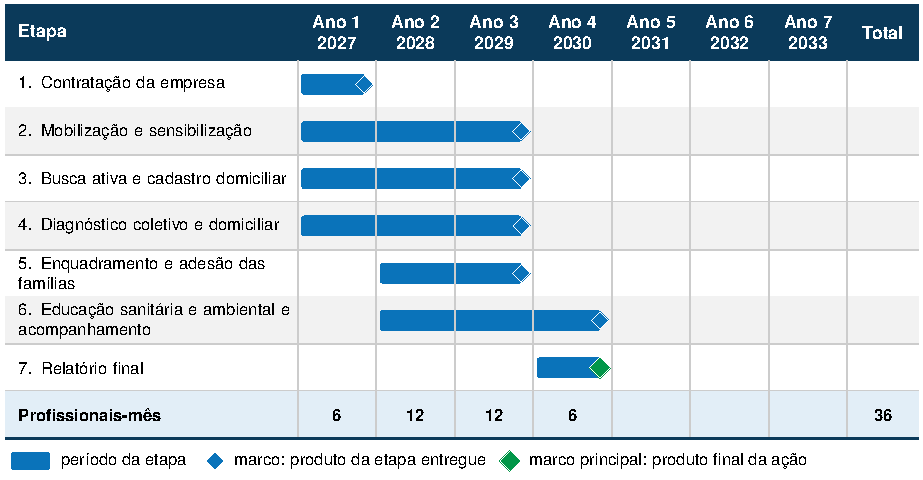
\includegraphics[width=15.64cm]{figuras/g-crono-3222.pdf}
  \fonteMOP{Fonte: IAT (2026), com quantidades da planilha PSH\_CUSTO\_Consolidada (PARANÁ, 2026).}
  % Texto alternativo: Cronograma anual de 2027 a 2033 com as etapas e as quantidades a entregar do trabalho técnico-social.
\end{figure}

\pendencia{O trabalho técnico-social encerra-se em 2030, e as obras de abastecimento e de esgotamento sanitário prosseguem até 2033. Avaliar se o acompanhamento social das obras de 2031 a 2033 requer recursos adicionais ou se será realizado pela equipe do IAT e pelas unidades regionais.}

\phantomsection
\addcontentsline{toc}{subsection}{9. Interfaces e dependências}
\subsection*{9. Interfaces e dependências}

A ação recebe dos modelos de gestão os municípios aderidos e os Termos de Cooperação e, da implantação dos sistemas de abastecimento, o cronograma das obras. Fornece o cadastro e as adesões que dão origem às associações, o diagnóstico que subsidia os projetos de abastecimento e a relação de domicílios sem esgotamento sanitário adequado (Figura~\ref{interf-3222}).

\begin{figure}[H]
  \centering
  \caption{Interfaces e dependências do trabalho técnico-social}\label{interf-3222}
  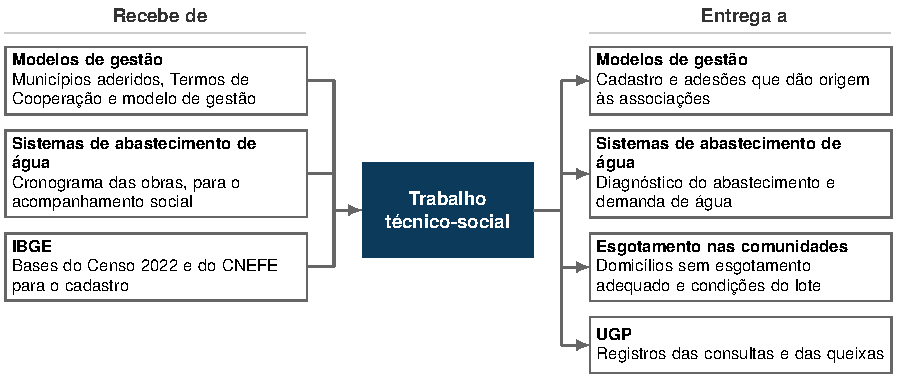
\includegraphics[width=15.30cm]{figuras/g-interf-3222.pdf}
  \fonteMOP{Fonte: IAT (2026).}
  % Texto alternativo: Diagrama das interfaces do trabalho técnico-social: insumos recebidos de outras partes do Programa e produtos entregues a elas.
\end{figure}

\phantomsection
\addcontentsline{toc}{subsection}{10. Documentos complementares}
\subsection*{10. Documentos complementares}

\begin{itemize}
  \item Termo de Referência do trabalho técnico-social (a elaborar);
  \item Termo de Cooperação entre o IAT e cada município;
  \item Plano de Engajamento das Partes Interessadas (PEPI) e Mecanismo de Queixas e Reclamações, no Caderno AS;
  \item Lei nº~13.709/2018 (Lei Geral de Proteção de Dados Pessoais);
  \item Programa Nacional de Saneamento Rural (BRASIL, 2019);
  \item Caderno AQ.
\end{itemize}
